% Options for packages loaded elsewhere
\PassOptionsToPackage{unicode}{hyperref}
\PassOptionsToPackage{hyphens}{url}
%
\documentclass[
]{article}
\usepackage{lmodern}
\usepackage{amsmath}
\usepackage{ifxetex,ifluatex}
\ifnum 0\ifxetex 1\fi\ifluatex 1\fi=0 % if pdftex
  \usepackage[T1]{fontenc}
  \usepackage[utf8]{inputenc}
  \usepackage{textcomp} % provide euro and other symbols
  \usepackage{amssymb}
\else % if luatex or xetex
  \usepackage{unicode-math}
  \defaultfontfeatures{Scale=MatchLowercase}
  \defaultfontfeatures[\rmfamily]{Ligatures=TeX,Scale=1}
\fi
% Use upquote if available, for straight quotes in verbatim environments
\IfFileExists{upquote.sty}{\usepackage{upquote}}{}
\IfFileExists{microtype.sty}{% use microtype if available
  \usepackage[]{microtype}
  \UseMicrotypeSet[protrusion]{basicmath} % disable protrusion for tt fonts
}{}
\makeatletter
\@ifundefined{KOMAClassName}{% if non-KOMA class
  \IfFileExists{parskip.sty}{%
    \usepackage{parskip}
  }{% else
    \setlength{\parindent}{0pt}
    \setlength{\parskip}{6pt plus 2pt minus 1pt}}
}{% if KOMA class
  \KOMAoptions{parskip=half}}
\makeatother
\usepackage{xcolor}
\IfFileExists{xurl.sty}{\usepackage{xurl}}{} % add URL line breaks if available
\IfFileExists{bookmark.sty}{\usepackage{bookmark}}{\usepackage{hyperref}}
\hypersetup{
  pdftitle={Working with R Utility Software},
  pdfauthor={Bill Venables},
  hidelinks,
  pdfcreator={LaTeX via pandoc}}
\urlstyle{same} % disable monospaced font for URLs
\usepackage[margin=1in]{geometry}
\usepackage{color}
\usepackage{fancyvrb}
\newcommand{\VerbBar}{|}
\newcommand{\VERB}{\Verb[commandchars=\\\{\}]}
\DefineVerbatimEnvironment{Highlighting}{Verbatim}{commandchars=\\\{\}}
% Add ',fontsize=\small' for more characters per line
\usepackage{framed}
\definecolor{shadecolor}{RGB}{248,248,248}
\newenvironment{Shaded}{\begin{snugshade}}{\end{snugshade}}
\newcommand{\AlertTok}[1]{\textcolor[rgb]{0.94,0.16,0.16}{#1}}
\newcommand{\AnnotationTok}[1]{\textcolor[rgb]{0.56,0.35,0.01}{\textbf{\textit{#1}}}}
\newcommand{\AttributeTok}[1]{\textcolor[rgb]{0.77,0.63,0.00}{#1}}
\newcommand{\BaseNTok}[1]{\textcolor[rgb]{0.00,0.00,0.81}{#1}}
\newcommand{\BuiltInTok}[1]{#1}
\newcommand{\CharTok}[1]{\textcolor[rgb]{0.31,0.60,0.02}{#1}}
\newcommand{\CommentTok}[1]{\textcolor[rgb]{0.56,0.35,0.01}{\textit{#1}}}
\newcommand{\CommentVarTok}[1]{\textcolor[rgb]{0.56,0.35,0.01}{\textbf{\textit{#1}}}}
\newcommand{\ConstantTok}[1]{\textcolor[rgb]{0.00,0.00,0.00}{#1}}
\newcommand{\ControlFlowTok}[1]{\textcolor[rgb]{0.13,0.29,0.53}{\textbf{#1}}}
\newcommand{\DataTypeTok}[1]{\textcolor[rgb]{0.13,0.29,0.53}{#1}}
\newcommand{\DecValTok}[1]{\textcolor[rgb]{0.00,0.00,0.81}{#1}}
\newcommand{\DocumentationTok}[1]{\textcolor[rgb]{0.56,0.35,0.01}{\textbf{\textit{#1}}}}
\newcommand{\ErrorTok}[1]{\textcolor[rgb]{0.64,0.00,0.00}{\textbf{#1}}}
\newcommand{\ExtensionTok}[1]{#1}
\newcommand{\FloatTok}[1]{\textcolor[rgb]{0.00,0.00,0.81}{#1}}
\newcommand{\FunctionTok}[1]{\textcolor[rgb]{0.00,0.00,0.00}{#1}}
\newcommand{\ImportTok}[1]{#1}
\newcommand{\InformationTok}[1]{\textcolor[rgb]{0.56,0.35,0.01}{\textbf{\textit{#1}}}}
\newcommand{\KeywordTok}[1]{\textcolor[rgb]{0.13,0.29,0.53}{\textbf{#1}}}
\newcommand{\NormalTok}[1]{#1}
\newcommand{\OperatorTok}[1]{\textcolor[rgb]{0.81,0.36,0.00}{\textbf{#1}}}
\newcommand{\OtherTok}[1]{\textcolor[rgb]{0.56,0.35,0.01}{#1}}
\newcommand{\PreprocessorTok}[1]{\textcolor[rgb]{0.56,0.35,0.01}{\textit{#1}}}
\newcommand{\RegionMarkerTok}[1]{#1}
\newcommand{\SpecialCharTok}[1]{\textcolor[rgb]{0.00,0.00,0.00}{#1}}
\newcommand{\SpecialStringTok}[1]{\textcolor[rgb]{0.31,0.60,0.02}{#1}}
\newcommand{\StringTok}[1]{\textcolor[rgb]{0.31,0.60,0.02}{#1}}
\newcommand{\VariableTok}[1]{\textcolor[rgb]{0.00,0.00,0.00}{#1}}
\newcommand{\VerbatimStringTok}[1]{\textcolor[rgb]{0.31,0.60,0.02}{#1}}
\newcommand{\WarningTok}[1]{\textcolor[rgb]{0.56,0.35,0.01}{\textbf{\textit{#1}}}}
\usepackage{longtable,booktabs}
\usepackage{calc} % for calculating minipage widths
% Correct order of tables after \paragraph or \subparagraph
\usepackage{etoolbox}
\makeatletter
\patchcmd\longtable{\par}{\if@noskipsec\mbox{}\fi\par}{}{}
\makeatother
% Allow footnotes in longtable head/foot
\IfFileExists{footnotehyper.sty}{\usepackage{footnotehyper}}{\usepackage{footnote}}
\makesavenoteenv{longtable}
\usepackage{graphicx}
\makeatletter
\def\maxwidth{\ifdim\Gin@nat@width>\linewidth\linewidth\else\Gin@nat@width\fi}
\def\maxheight{\ifdim\Gin@nat@height>\textheight\textheight\else\Gin@nat@height\fi}
\makeatother
% Scale images if necessary, so that they will not overflow the page
% margins by default, and it is still possible to overwrite the defaults
% using explicit options in \includegraphics[width, height, ...]{}
\setkeys{Gin}{width=\maxwidth,height=\maxheight,keepaspectratio}
% Set default figure placement to htbp
\makeatletter
\def\fps@figure{htbp}
\makeatother
\setlength{\emergencystretch}{3em} % prevent overfull lines
\providecommand{\tightlist}{%
  \setlength{\itemsep}{0pt}\setlength{\parskip}{0pt}}
\setcounter{secnumdepth}{-\maxdimen} % remove section numbering
\usepackage[utf8]{inputenc}
\usepackage{fullpage,parskip,fouriernc}
\ifluatex
  \usepackage{selnolig}  % disable illegal ligatures
\fi

\title{Working with R Utility Software}
\author{Bill Venables}
\date{2020-12-28}

\begin{document}
\maketitle

{
\setcounter{tocdepth}{3}
\tableofcontents
}
\hypertarget{introduction}{%
\section{Introduction}\label{introduction}}

Vignettes are long form documentation commonly included in packages.
Because they are part of the distribution of the package, they need to
be as compact as possible. The \texttt{html\_vignette} output type
provides a custom style sheet (and tweaks some options) to ensure that
the resulting html is as small as possible. The \texttt{html\_vignette}
format:

\begin{itemize}
\tightlist
\item
  Never uses retina figures
\item
  Has a smaller default figure size
\item
  Uses a custom CSS stylesheet instead of the default Twitter Bootstrap
  style
\end{itemize}

\hypertarget{vignette-info}{%
\subsection{Vignette Info}\label{vignette-info}}

Note the various macros within the \texttt{vignette} section of the
metadata block above. These are required in order to instruct R how to
build the vignette. Note that you should change the \texttt{title} field
and the \texttt{\textbackslash{}VignetteIndexEntry} to match the title
of your vignette.

\hypertarget{styles}{%
\subsection{Styles}\label{styles}}

The \texttt{html\_vignette} template includes a basic CSS theme. To
override this theme you can specify your own CSS in the document
metadata as follows:

\begin{verbatim}
output: 
  rmarkdown::html_vignette:
    css: mystyles.css
\end{verbatim}

\hypertarget{figures}{%
\subsection{Figures}\label{figures}}

The figure sizes have been customised so that you can easily put two
images side-by-side.

\begin{Shaded}
\begin{Highlighting}[]
\NormalTok{lazyData}\SpecialCharTok{::}\FunctionTok{requireData}\NormalTok{(doParallel)}
\FunctionTok{par}\NormalTok{(}\AttributeTok{mar=}\FunctionTok{c}\NormalTok{(}\DecValTok{1}\NormalTok{,}\DecValTok{1}\NormalTok{,}\DecValTok{4}\NormalTok{,}\DecValTok{1}\NormalTok{), }\AttributeTok{mfrow =} \FunctionTok{c}\NormalTok{(}\DecValTok{2}\NormalTok{,}\DecValTok{2}\NormalTok{))}
\NormalTok{pals }\OtherTok{\textless{}{-}} \FunctionTok{paste0}\NormalTok{(}\StringTok{"pal\_"}\NormalTok{, }\FunctionTok{cq}\NormalTok{(desert, green2pink, blue2red, heat\_hcl))}
\FunctionTok{foreach}\NormalTok{(}\AttributeTok{pal =}\NormalTok{ pals, }\AttributeTok{let =}\NormalTok{ letters[}\DecValTok{1}\SpecialCharTok{:}\DecValTok{4}\NormalTok{]) }\SpecialCharTok{\%do\%}\NormalTok{ \{}
  \FunctionTok{showColors}\NormalTok{(}\FunctionTok{get}\NormalTok{(pal)(}\DecValTok{150}\NormalTok{), }\AttributeTok{main =}\NormalTok{ pal)}
  \FunctionTok{text}\NormalTok{(}\StringTok{"top right"}\NormalTok{, }\FunctionTok{paste0}\NormalTok{(}\StringTok{"("}\NormalTok{, let, }\StringTok{")"}\NormalTok{), }\AttributeTok{cex =} \FloatTok{1.25}\NormalTok{, }\AttributeTok{font =} \DecValTok{2}\NormalTok{)}
\NormalTok{\} }\SpecialCharTok{\%\textgreater{}\%} \FunctionTok{invisible}\NormalTok{()}
\end{Highlighting}
\end{Shaded}

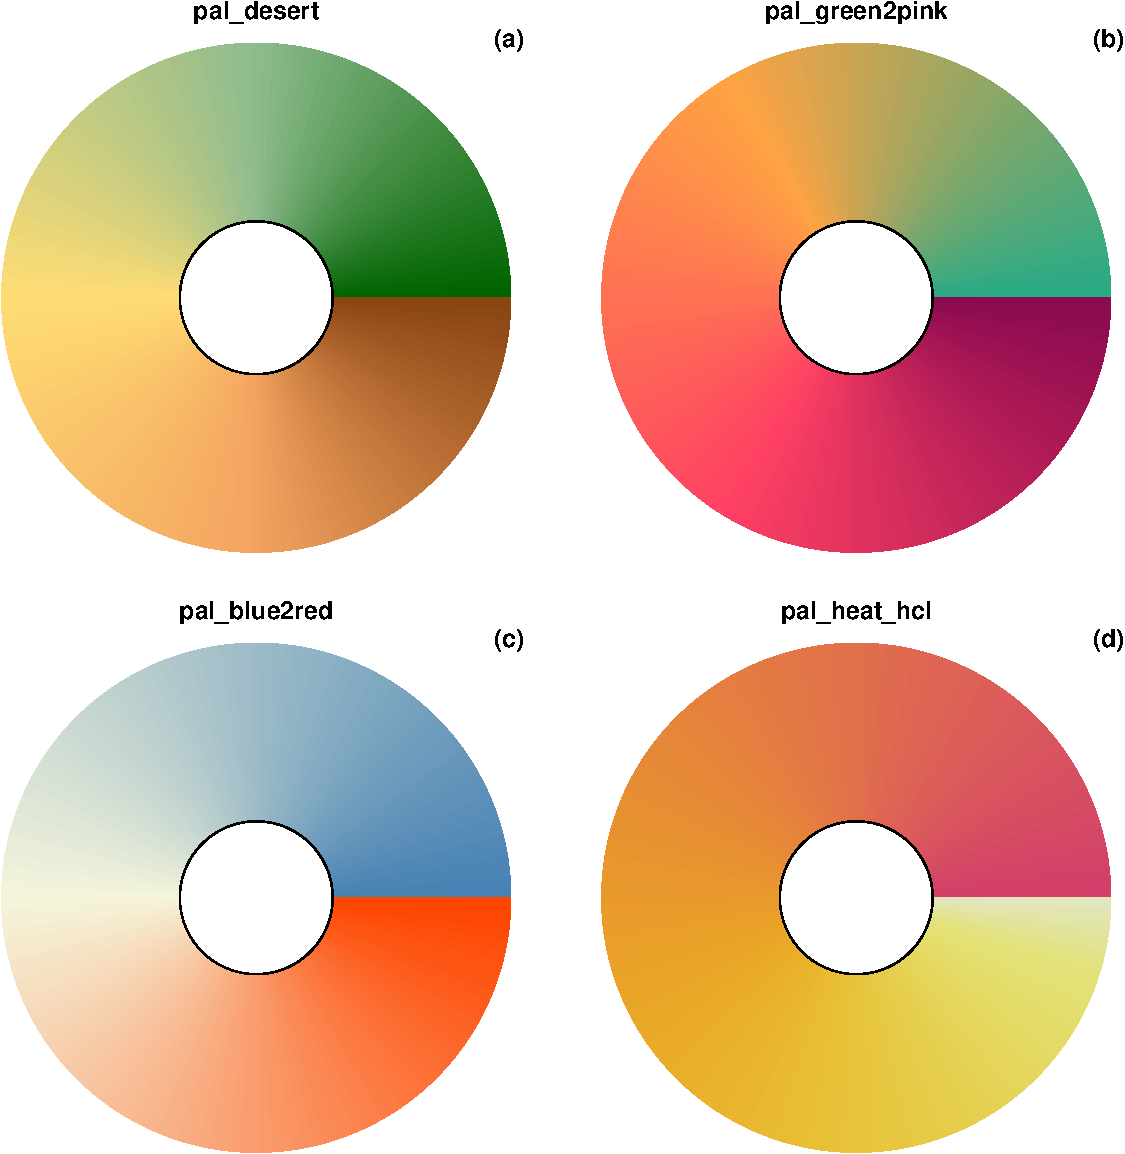
\includegraphics[width=0.8\textwidth]{/home/ven037/Dropbox/R/Git/WWRGraphics/vignettes/working_with_r_files/figure-latex/unnamed-chunk-1-1}

You can enable figure captions by \texttt{fig\_caption:\ yes} in YAML:

\begin{verbatim}
output:
  rmarkdown::html_vignette:
    fig_caption: yes
\end{verbatim}

Then you can use the chunk option
\texttt{fig.cap\ =\ "Your\ figure\ caption."} in \textbf{knitr}.

\hypertarget{more-examples}{%
\subsection{More Examples}\label{more-examples}}

You can write math expressions, e.g.~\(Y = X\beta + \epsilon\),
footnotes\footnote{A footnote here.}, and tables, e.g.~using
\texttt{knitr::kable()}.

\begin{longtable}[]{@{}lrrrrrrrrrrr@{}}
\toprule
& mpg & cyl & disp & hp & drat & wt & qsec & vs & am & gear &
carb\tabularnewline
\midrule
\endhead
Mazda RX4 & 21.0 & 6 & 160.0 & 110 & 3.90 & 2.620 & 16.46 & 0 & 1 & 4 &
4\tabularnewline
Mazda RX4 Wag & 21.0 & 6 & 160.0 & 110 & 3.90 & 2.875 & 17.02 & 0 & 1 &
4 & 4\tabularnewline
Datsun 710 & 22.8 & 4 & 108.0 & 93 & 3.85 & 2.320 & 18.61 & 1 & 1 & 4 &
1\tabularnewline
Hornet 4 Drive & 21.4 & 6 & 258.0 & 110 & 3.08 & 3.215 & 19.44 & 1 & 0 &
3 & 1\tabularnewline
Hornet Sportabout & 18.7 & 8 & 360.0 & 175 & 3.15 & 3.440 & 17.02 & 0 &
0 & 3 & 2\tabularnewline
Valiant & 18.1 & 6 & 225.0 & 105 & 2.76 & 3.460 & 20.22 & 1 & 0 & 3 &
1\tabularnewline
Duster 360 & 14.3 & 8 & 360.0 & 245 & 3.21 & 3.570 & 15.84 & 0 & 0 & 3 &
4\tabularnewline
Merc 240D & 24.4 & 4 & 146.7 & 62 & 3.69 & 3.190 & 20.00 & 1 & 0 & 4 &
2\tabularnewline
Merc 230 & 22.8 & 4 & 140.8 & 95 & 3.92 & 3.150 & 22.90 & 1 & 0 & 4 &
2\tabularnewline
Merc 280 & 19.2 & 6 & 167.6 & 123 & 3.92 & 3.440 & 18.30 & 1 & 0 & 4 &
4\tabularnewline
\bottomrule
\end{longtable}

Also a quote using \texttt{\textgreater{}}:

\begin{quote}
``He who gives up {[}code{]} safety for {[}code{]} speed deserves
neither.''
(\href{https://twitter.com/hadleywickham/status/504368538874703872}{via})
\end{quote}

\end{document}
